
%(BEGIN_QUESTION)
% Copyright 2011, Tony R. Kuphaldt, released under the Creative Commons Attribution License (v 1.0)
% This means you may do almost anything with this work of mine, so long as you give me proper credit

Forutsi effekten av at dampflowtransmitteren plutselig feiler høyt (20 mA). Anta korrekt konfigurerte komponenter, godt tunet regulator og at systemet har fått tid til å stabilisere seg:

$$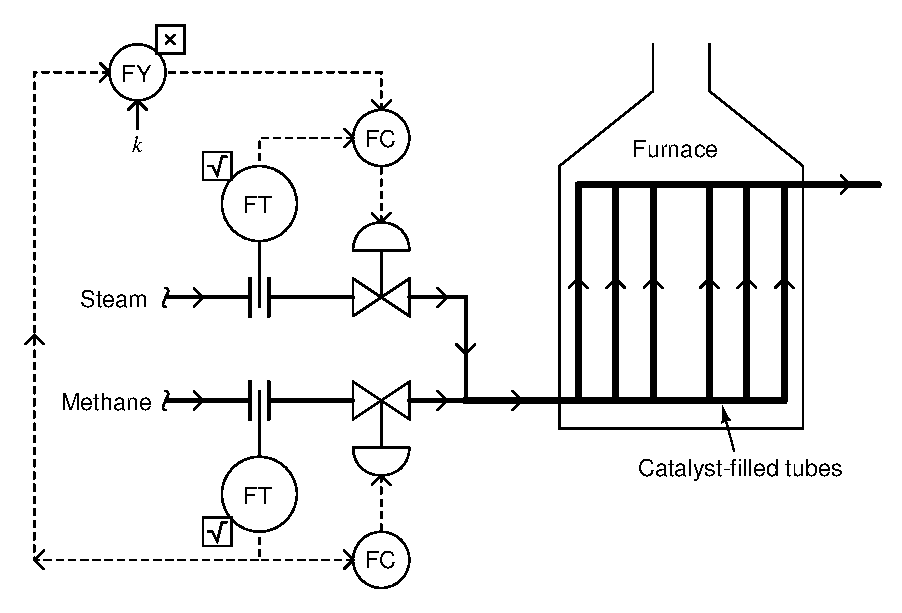
\includegraphics[width=15.5cm]{i00980x01.eps}$$

\begin{itemize}
\item{} Dampventilen vil: {\it åpne mer}, {\it lukke mer}, eller {\it være uendret}
\vskip 10pt
\item{} Metanventilen vil: {\it åpne mer}, {\it lukke mer}, eller {\it være uendret}
\end{itemize}

\underbar{file i00980}
%(END_QUESTION)





%(BEGIN_ANSWER)

\begin{itemize}
\item{} Dampventilen vil: {\bf lukke mer}
\vskip 5pt
\item{} Metanventilen vil: {\bf være uendret}
\end{itemize}

%(END_ANSWER)





%(BEGIN_NOTES)

{\bf Denne oppgaven er ment kun for eksamen, ikke for arbeidsark!}.

%(END_NOTES)

